\documentclass{book}

\usepackage[T1,T2A]{fontenc}
\usepackage[utf8]{inputenc}
\usepackage[ukrainian]{babel}
\usepackage{makeidx}
\usepackage[unicode]{hyperref}
\usepackage[symbol]{footmisc}
\usepackage{marvosym}
\usepackage{amssymb}
\usepackage{graphicx}
\usepackage{caption}
\usepackage{subcaption}
\usepackage{environ}
\usepackage{tikz}
\usepackage{enumitem}

\title{Робимо програми: шлях хакера}
\author{А. Мустіц}
\date{\today}
\makeindex

\renewcommand{\thefootnote}{\fnsymbol{footnote}}
\NewEnviron{exercise}{\par\goodbreak\smallskip\textbf{Вправа:} \BODY \par\smallskip}
\NewEnviron{summary}{\par\goodbreak\smallskip\textbf{Підсумки:}\begin{itemize} \BODY \end{itemize}\par\smallskip}

\NewEnviron{algorithm}{\medskip\goodbreak \BODY \medskip\goodbreak}
%\NewEnviron{algsteps}{\begin{enumerate}[\hspace{2\parindent}1.] \BODY \end{enumerate}}
\NewEnviron{algsteps}{\begin{enumerate}[
  topsep=0pt,itemsep=-1ex,partopsep=1ex,parsep=1ex,
  leftmargin=3\parindent
  ] \BODY \end{enumerate}}
\newcommand{\algcaption}[1]{\textbf{Алгоритм:} #1.\par}
\newcommand{\alginput}[1]{\textbf{Дано:} #1\par}
\newcommand{\algoutput}[1]{\textbf{Треба:} #1\par}
\newcommand{\algstep}{\item}
\newcommand{\algsummary}[1]{\par\textbf{Результат:} #1\par}

\newcommand{\bitstr}[1]{{\tt #1}}
\newcommand{\bitdesc}{послідовність бітів ми будемо писати моноширинним шрифтом, наприклад запис \bitstr{10011} означатиме послідовність п'яти біт \bitstr{1}, \bitstr{0}, \bitstr{0}, \bitstr{1} та \bitstr{1}.}

\newcommand{\tritzero}{$\square$}
\newcommand{\trithalf}{\Yinyang}
\newcommand{\tritone}{$\blacksquare$}

\newcommand{\setunref}{\href{https://uk.wikipedia.org/wiki/\%D0\%A1\%D0\%B5\%D1\%82\%D1\%83\%D0\%BD\%D1\%8C_(\%D0\%BA\%D0\%BE\%D0\%BC\%D0\%BF\%27\%D1\%8E\%D1\%82\%D0\%B5\%D1\%80)}{https://uk.wikipedia.org/wiki/Сетунь\_(комп'ютер)}}
\newcommand{\quantumref}{\href{https://uk.wikipedia.org/wiki/\%D0\%9A\%D0\%B2\%D0\%B0\%D0\%BD\%D1\%82\%D0\%BE\%D0\%B2\%D0\%B8\%D0\%B9_\%D0\%BA\%D0\%BE\%D0\%BC\%D0\%BF\%27\%D1\%8E\%D1\%82\%D0\%B5\%D1\%80}{https://uk.wikipedia.org/wiki/Квантовий\_комп'ютер}}
\newcommand{\kruskalref}{\href{https://en.wikipedia.org/wiki/Kruskal\%27s_tree_theorem}{https://en.wikipedia.org/wiki/Kruskal\%27s\_tree\_theorem}}

\begin{document}

\maketitle
\chapter{TBD}
\section{TBD}
\subsection{Біти та інформація}

Що таке комп'ютерна програма?
Одне з визначень, яке можна дати, це певні інструкції, як обробляти інформацію.
Що призводить до не менш цікавого запитання: «А що тоді таке інформація?» \index{інформація}
Щоб дати ретельну відповідь на нього, треба написати не одну книжку.
Цей термін часто використовується у повсякденному житті, тому кожен має своє власне інтуїтивне уявлення, яке дуже важко пояснити словами.
Також інформація з'являється в математиці, фізиці, інформатиці, та у багатьох інших дисциплінах.
Як завжди, у кожному такому контексті цей термін обростає своїми особливими рисами та нюансами.

\begin{figure}[t]
  \centering
  \begin{subfigure}[b]{0.45\textwidth}
    \centering
    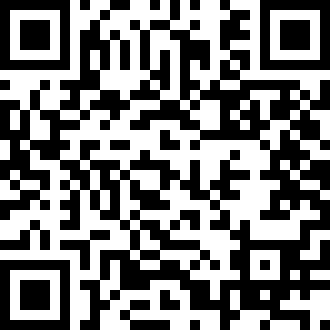
\includegraphics[width=\textwidth]{images/qr2.png}
    \caption{~}
    \label{Pic_QR_BW}
  \end{subfigure}
  \hfill
  \begin{subfigure}[b]{0.45\textwidth}
    \centering
    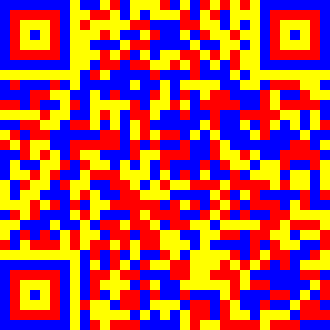
\includegraphics[width=\textwidth]{images/qr3.png}
    \caption{~}
    \label{Pic_QR_Color}
  \end{subfigure}
  \caption{На QR коді ми можемо на власні очі побачити біти (а); також показаний гіпотетичний QR код, який складається зі тритів (б).}
  \label{PicQR}
\end{figure}

Але я б хотів виділити один момент, який буде для нас важливим.
Інформація це часто є акцентування однієї з можливих альтернатив.
Наприклад, «Танєєв народився у 1856 році».\footnote{
  Приклад про Танєєва взятий з оповідання Іраклія Андронікова «Перший раз на естраді», яке можна прочитати в інтернеті або подивитися на youtube.
  \par\url{https://www.youtube.com/watch?v=dm8wdFKag94}}
Це означає, що Танєєв не міг народитися у 1858 році, 1859, 1860, 1861, 1862, і т.~д.
Тобто з усіх можливих альтернатив, коли міг народитися Танєєв, ми обираємо одну.
Цього погляду нам вистачить для потреб цієї книги.

Добре, тепер спробуємо поміркувати так, як це роблять програмісти та математики.
Який шмат інформації самий найпростіший?
Інтуїтивно, це вибір однієї з двох альтернатив.
Тому що три це вже забагато, а у разі однієї альтернативи мова не йде про вибір.
«Танєєв народився від батька та матері!»
Це викликає посмішку, бо незрозуміло, які є ще варіанти?
Так, з сучасними технологічними досягненнями у галузі біомедицини, у певному контексті ще можна уявити на чому саме робиться акцент, але не у 1856 році.

Сама дрібна одиниця інформація, а саме вибір однієї з двох альтернатив, називається бітом. \index{біт}
Це може бути орел чи решка, парне або непарне, біле або чорне, хрестик або нулик, \Male\ або \Female, живий або мертвий, уперед чи назад, правда чи брехня.

\begin{exercise}
Придумайте ще приклади інформації, які можна закодувати одним бітом.
\end{exercise}

У сучасній мікроелектроніці, біт це наявність або відсутність електричного сигналу за певний проміжок часу, який називається тактом. \index{такт}
Переважна кількість сучасних процесорів бачать увесь свій світ виключно як послідовність біт.
Коли ми на комп'ютері слухаємо музику, дивимося відео або граємо у 3D ігри, коли робиться автоматичний переклад з однієї мови на іншу, коли автоматично генеруються пейзажі, то інколи дуже важко повірити в те, що віртуальна реальність складається виключно з бітів, але це так.
Однією нашою метою буде як раз пояснення того, як реальний світ може бути змодельований з бітів.

Проте, поширення електронних пристроїв призвело до того, що ми можемо фізично побачити біти навіть у реальному житті.
Гарний приклад цього це QR~коди, де біти видно на власні очі (рис.~\ref{Pic_QR_BW}).
Тут чорні квадратики кодують один стан, а білі---інший.

Оскільки ми будемо вести багато розмов про біти, було б добре їх якось позначати.
Біт може бути у одному з двох станів, тому для цього можна вибрати два будь-яких символи, наприклад $\blacksquare$ та $\square$, як на QR~коді.
Але історично в математиці для цього використовуються числа $0$ та $1$.
Щоб відрізняти звичайні десяткові числа, складені з нулів та одиниць, наприклад, як  $101$ (сто один),  від послідовності біт \bitstr{1}, \bitstr{0} та \bitstr{1}, ми будемо триматися наступних домовленостей:
\bitdesc

За визначенням, один біт може кодувати два різних варіанти. А скільки варіантів кодує два біти? Нескладно порахувати, що відповідь на це запитання буде чотири, ось усі варіанти: \bitstr{00}, \bitstr{01}, \bitstr{10} та \bitstr{11}. Взагалі, якщо ми збільшуємо кількість біт на один, то кількість варіантів зростає у двічі.
Це легко пояснити тим, що для будь якого попередньої комбінації ми можемо додати або біт \bitstr{0}, або біт \bitstr{1}.
Загально, якщо в нас є $n$ біт, то з них можна скласти $2^n$ різних комбінацій.

\begin{exercise}
Побудуйте усі різні комбінації, які можна створити з трьох біт.
\end{exercise}

\begin{exercise}
Скільки усього можливих комбінацій можна скласти з $10$ біт?
\end{exercise}

Я сподіваюся, що до цього моменту ви вже розібралися, що таке біти.
Тому настав час трохи відпочити та пофлудити.
Отже, біт має два стани, які ми позначаємо \bitstr{0} та \bitstr{1}.
Також ми відмітили, що безглуздо розглядати щось, що має лише один стан.
А якщо розглянути систему, яка має три стани, наприклад \tritzero, \tritone\ та \trithalf?
\index{тріт} Назвемо трітом одиницю інформації, де у нас є вибір з трьох альтернатив.

\begin{exercise}
Побудуйте усі різні комбінації, які можна створити з двох тритів.
\end{exercise}

Чи дасть це нам якісь переваги?
З математичної точки зору, усе що можна представити з тритів, можна представити й за допомогою бітів.
Самий простий шлях це зробити просто використовувати два біти для кодування одного тріта: \bitstr{00}~—~\tritzero, \bitstr{11}~—~\tritone\ та \bitstr{01}~—~\trithalf.
Так, звичайно комбінація \bitstr{10} не буде використовуватися.
Так, звичайно бітів буде вдвічі більше ніж тритів.
Але коли це хвилювало математиків?

\begin{exercise}
Скільки біт треба для того, щоб закодувати інформацію, яка міститься у двох трітах?
Скільки комбінацій при цьому не буде використано?
\end{exercise}

Добре, а що з точки зору народного господарства?
Якщо зберігати інформацію у трітах замість бітів, чи не виграємо ми додаткове місце?
Яке не яке, а досягнення.
Але, на практиці усе не так просто.
Безкоштовний газ є тільки у газовій камері.

Подивимося на рис.~\ref{Pic_QR_Color}.
На ньому я намагався нафантазувати, як би мав виглядати QR~код з тритів.
Замість чорної та білої фарб, використано жовту, синю та червоні фарби.
Ніби то виграш є?
Але на практиці розрізняти три фарби складніше.
Тому у звичайному чорно-білому варіанті ми зможемо розрізняти менші квадратики, а це також буде впливати на щільність запису інформацію.

Зробити процесори, які працюють з трітами, не питання.
За радянських часів була побудована ЕОМ Сетунь\footnote{\setunref}, яка працювала з трітами. \index{Сетунь}
Розрізнялися не тільки наявність та відсутність сигналу, але й його напрямок.
Хтось й по сьогоднішній день вважає це революційним досягненням, але я до цього ставлюся скептично.
Проектування процесорів зараз суто технічний процес.
Е багато інструментів, програмних застосунків, які дозволяють моделювати нові процесори.
Цим займається багато спеціалістів по усьому світу, тому усе що можна було перепробувати, вони вже перепробували.
Отже, якщо переважна більшість сучасних комп'ютерів працюють з бітами, то це означає, що не зважаючи на свою привабливість, тріти все ж таки програють бітам.

Але, там де це доречно, то чому б не розглянути?
У WiFi інформація передається символами, кожен з яких може нести величезну кількість варіантів.
Так, оскільки ця інформація у евентуально буде оброблятися звичайним процесором, то з практичної точки зору цю кількість варіантів намагаються зробити ступенями двійки.
Це дає змогу казати, що один символ несе $1024$ біти інформації.
Але у самій електромагнітній хвилі важко побачити окремі біти.

Також скажу декілька слів про квантові обчислення, кубіти, або квантові біти. \index{кубіт}
Так, на сьогодні віртуальний світ складається з бітів. А що у реальному?
Якщо опуститися на рівень квантових взаємодій, ми побачимо, що там працюють свої екзотичні контрінтуїтивні закони.
Окрім двох альтернатив, які виключають одна одну, ми часто бачимо їх суперпозицію.
Наприклад, електрон на $30$\% обертається праворуч, а на $70$\%---ліворуч.
Нам це важко уявити, але математичні формули працюють саме так.
Замість нуля та одиниці, ми отримуємо фізичну величину від нуля до одиниці.
Додайте ще фазу від нуля до $2\pi$, й ви отримаєте кубіт.
А ще суперпозиція станів, зворотні операції, вимірювання...

Вже з'являються перші квантові комп'ютери, які оперують кубітами.
Це може бути новою революцією.
Але на початку все ж таки краще освоїти звичайне програмування, яке працює з бітами.
А вже потім переходити до квантового.

\begin{exercise}
Продивиться статтю у Wikiepedia про квантові комп'ютери\footnote{\quantumref}. Чи це цікаво?
\end{exercise}

\begin{summary}
\item Інформація вимірюється у бітах.  Біт це найменший шмат інформації, який складається з двох станів, які позначаються \bitstr{0} та \bitstr{1}.
\item З $n$ біт можна скласти $2^n$ різних комбінацій.
\end{summary}

\subsection{Числа, скільки біт нам вистачить?}

Відомий німецький математик Леопольд Кронекер якось казав: «Бог створив натуральні числа, решта — справа рук людини».
Числа відіграють дуже важливу роль в нашому житті, тому розглянемо, як можна складати з біт натуральні числа.
Але, на превеликий жаль, точна відповідь на це запитання «Ніяк».
Натуральних чисел нескінченна кількість, тому скільки би ми не брали бітів, все одно з них можна буде скласти лише обмежену кількість різних комбінацій.

Але, якщо підійти до цієї проблеми не з точки зору теорії, а з боку потреб народного господарства, то як часто ми маємо проблему працювати з величезними числами?
Як часто у повсякденному житті ми чуємо про квадрильйони, та секстильйони?

\begin{exercise}
Скільки нулів наприкінці в записі чисел «один квадрильйон» та «один секстильйон»?
\end{exercise}

Тому заслуговує уваги практичний спосіб вирішення проблеми, коли ми кодуємо не усі натуральні числа, а до деякого числа, яке нам здається розумним обмеженням.
Якщо для збереження натурального числа виділити $n$ біт, то, як ми вже знаємо, ми зможемо зберігати $2^n$ різних комбінацій.
Оскільки перше число, яке ми будемо зберігати, це $0$, то останнє число буде $2^n-1$.
Оцінимо тепер різні значення $n$, які часто зустрічаються на практиці.

Припустимо, $n=8$. Як ми дізнаємося пізніше, це байт.
Таким чином ми можемо зберігати числа від $0$ до $255$.
Такий діапазон покриває лише невеличку частину потреб.
Наприклад, у восьмі бітах ми можемо зберігати кількість дітей, пульс (кількість ударів за хвилину), кількість сторінок у зошиті, кількість кнопок у миші, і~т.~д.
Але для зберігання більшості чисел, з якими ми зустрічаємося на практиці, цього буде недостатньо.

\begin{exercise}
Придумайте ще значення, які можна зберігати у восьми бітах
\end{exercise}

У $2010$-х роках була популярна $32$-бітна архітектура.
Цієї кількості біт вистачає для збереження чисел від $0$ до $4~294~967~295$.
Цього вже достатньо для багатьох практичних потреб, будь то заробітна платня або кількість книг у бібліотеці.
Але все ж таки існують й виключення, наприклад борг державного департаменту США, або населення земної кулі.

\begin{exercise}
Для збереження яких ще значень не вистачить $32$-х біт?
\end{exercise}

Тут може виникати запитання, можемо чи ми працювати з $64$-х, або навіть з $128$-ми бітними числами, якщо у нас $32$-бітний процесор.
Відповідь на це запитання проста: можемо, але це буде повільніше.
Бітність процесора означає, над якими числами дії будуть виконуватися за одну операцію.
Щоб працювати з числами з більшою кількістю бітів, нам треба буде написати або використати готові програми, які будуть виконувати потрібні дії але за більшу кількість елементарних операцій.

Зараз більшість комп'ютерів має $64$-бітну архітектуру, таким чином діапазон складає від $0$ до запаморочливого числа $18~446~744~073~709~551~615$, яке вимовляється «18 квінтильйонів, 446 квадрильйона, ...»
Як часто у житті ви оперуєте такими числам? Особисто я не часто.
Цікаво, що це число з'являється у притчі про раджу та винахідника шахів, який у нагороду попросив трохи зерна, одне на першу клітину, два на другу, чотири на третю,~...
На шахівниці усього $64$ клітини, тому  не дивно, що ці числа збіглися.

Але це ще не кінець.
Розробники криптовалюти Ethereum, платформи для смарт-контрактів, вибрали для своєї архітектури $512$ біт.\index{Ethereum}
Цього достатньо, щоб зберігати числа, які складаються зі $150$-ти цифр, а це більше ніж гугол, число $1^{100}$ або одиниця та сто нулів!
Вибір такого числа пояснюється тим, що зробити підтримку для мікротранзакцій з сумами значно менше ніж один цент.
$1$~wei, найдрібніше значення криптовалюти ETH, яким можна оперувати, на момент написання книги коштувало $0.000~000~000~000 002~598$ доларів.
Але головною причиною вибору такого значення був все ж таки технічний момент.
Автори Ethereum вибрали алгоритм хешування, який повертає $512$-бітне число.

Скажемо пару слів про хешування, та чому саме для нього потрібні такі величезні числа.\index{хеш}
Алгоритм хешування полягає у тому, щоб задану послідовність біт перетворити у певне обмежене число, яке називається хешем цієї послідовності.
Хешування є криптографічним, якщо \textit{практично неможливо}\footnote{
  Це означає, що сьогодні ніхто не наблизився до розв'язку цієї задачі.
  Або, якщо використовувати сучасні алгоритми, та усю планету перетворити на велетенський процесор, то потрібні будуть квінтильйони років для розв'язку.
} по хешу знайти послідовність біт, з якого він був згенерований, чи згенерувати дві послідовності, яким буде відповідати один й той самий хеш.
Таким чином, наприклад, дві сторони можуть опублікувати, що вони підписали договір, та надати його хеш.
Тоді ніхто не буде знати, який саме договір підписали сторони.
Але кожна зі сторін, наприклад у разі виникнення спору, може показати у суді договір, який відповідає хешу.
Ця техніка зазвичай дуже важлива для блокчейна.
Але якщо вибрати у якості хешу $32$-бітне число, то можна просто перебрати трохи більше $4$~млрд. різних послідовностей та знайти дві з однаковим хешем.
Чим більше біт, тим складніше перебирати та знаходити слабкі місця у алгоритмі.
Як раз $256$ та $512$-бітні хеші на сьогодні є компромісом між безпекою та швидкодією.

Далі йдуть цифрові підписи та шифрування.
Там компроміс між безпекою та швидкодією приводить нас до $1024$ або $2048$-бітного шифрування.
Але й інколи в деяких країнах у це втручається навіть закон, який обмежує кількість біт, які мають використовуватися для шифрування.
Напевне, щоб влада могла розшифрувати, якщо їй дуже сильно закортить.

Добре, припустимо ми виділили із запасом мільйон біт.
Думаєте цього усім вистачить?
Помиляєтеся, та дуже недооцінюєте математиків!
Вони дійшли до таких чисел, що навіть якщо для виділити усі диски у світі, все рівно їх не вистачить для зберігання навіть одного числа!
Прикладом такого числа є $TREE(3)$ з теореми Крускала\footnote{\kruskalref}.

\begin{summary}
\item Натуральних чисел нескінчена кількість, тому на практиці обмежуються деяким числом, яке, здається, неможливо перебільшити.
\item Чим більше біт використовується, тим більше потреб покривається, але тим повільніші операції. $64$-біт вистачає для більшості потреб.
\item Математики---божевільні!
\end{summary}

\subsection{Як скласти числа з біт?}

Добре, ми трохи обговорили тему, скільки біт треба виділити на числа у разі тієї чи іншої задачі.
Тепер треба вирішити більш практичне запитання: «Яким методом можна скласти числа з біт?» (рис.~\ref{Pic_Num_From_Bits})

\begin{figure}[t]
  \centering
  \begin{tikzpicture}
  % \draw[help lines] (0,0) grid (7,3);

  \node at (0.5,2.8) {$0$};
  \node at (1.0,2.8) {$1$};
  \node at (1.5,2.8) {$2$};
  \node at (2.0,2.8) {$3$};
  \node at (2.5,2.8) {$4$};
  \node at (3.0,2.8) {$5$};
  \node at (3.5,2.8) {$6$};
  \node at (4.0,2.8) {$7$};

  \node at (0.6, 0.2) {\bitstr{000}};
  \node at (1.6, 0.2) {\bitstr{001}};
  \node at (2.6, 0.2) {\bitstr{010}};
  \node at (3.6, 0.2) {\bitstr{100}};
  \node at (4.6, 0.2) {\bitstr{011}};
  \node at (5.6, 0.2) {\bitstr{101}};
  \node at (6.6, 1.0) {\bitstr{110}};
  \node at (6.6, 1.8) {\bitstr{111}};

  \draw (0.5,2.65)
    to [out=-90,in=180] (2.5, 0.7)
    to [out=0,in=-135] (3.5, 1.5)
    ;

  \draw (1.0,2.65)
    to [out=-90,in=180] (2.5, 2)
    to [out=0,in=135] (3.5, 1.5)
    ;

  \draw (1.5,2.65)
    to [out=-90,in=180] (2.8, 1.0)
    to [out=0,in=180] (3.5, 1.5)
    ;

  \draw (2.0,2.65)
    to [out=-90,in=180] (2.8, 1.8)
    to [out=0,in=180] (3.5, 1.5)
    ;

  \draw (2.5,2.65)
    to [out=-90,in=180] (3.0, 1.6)
    to [out=0,in=-135] (3.5, 1.5)
    ;

  \draw (3.0,2.65)
    to [out=-90,in=-90] (3.5, 1.5)
    ;

  \draw (3.5,2.65)
    to [out=-90,in=-90] (3.5, 1.5)
    ;

  \draw (4.0,2.65)
    to [out=-90,in=-80] (3.5, 1.5)
    ;

  \draw (0.6,0.35)
    to [out=90,in=180] (1.5, 1.8)
    to [out=0,in=-170] (3.5, 1.5)
    ;

  \draw (1.6,0.35)
    to [out=90,in=170] (2.5, 1.4)
    to [out=0,in=-150] (3.5, 1.5)
    ;

  \draw (2.6,0.35)
    to [out=90,in=-166] (3.5, 1.5)
    ;

  \draw (3.6,0.35)
    to [out=90,in=-90] (3.5, 1.5)
    ;

  \draw (4.6,0.35)
    to [out=90,in=-60] (3.5, 1.5)
    ;

  \draw (5.6,0.35)
    to [out=90,in=-30] (3.5, 1.5)
    ;

  \draw (6.3,1.0)
    to [out=180,in=10] (3.5, 1.5)
    ;

  \draw (6.3,1.8)
    to [out=180,in=30] (3.5, 1.5)
    ;

  \draw [fill=white] (3.5,1.5) circle [radius=0.5];
  \node at (3.5, 1.5) {?};

\end{tikzpicture}

  \caption{Яким саме послідовностям біт мають відповідати числа?}
  \label{Pic_Num_From_Bits}
\end{figure}

Знову, як математики та програмісти, на початку спробуємо розглянути самий елементарний випадок, а саме один єдиний біт.
Отже, у нас $n=1$, у нас є послідовності \bitstr{0} та \bitstr{1}.
Нам треба зіставити цим послідовностям числа $0$ та $1$.
Яким чином це можна зробити?
Сподіваюся, що якщо ви не диверсант, то вибрали природній шлях нуль назвати нулем, а одиницю---одиницею.

Тепер спробуємо розглянути випадок $n=2$.
Тепер ми маємо послідовності \bitstr{00}, \bitstr{01}, \bitstr{10}, \bitstr{11}, та числа $0$, $1$, $2$, $3$.
Тут гарно пригадати властивості звичайних чисел, а саме що до будь-якого числа можна зліва приписати будь яку кількість нулів, воно від цього не зміниться: $42 = 042 = 00042$.
Це дуже зручно на практиці, бо не треба гадати, як число з чотирьох біт перевести у число з восьми бітами: просто дописуємо потрібну кількість нулів.
Таким чином, ми вже маємо, що \bitstr{00} це $0$, а \bitstr{01} це $1$.
Лишилося лише знайти відповідність між \bitstr{10} й \bitstr{11}, ти числами $2$ і $3$.

І знову два способи це зробити: перший, коли $2$ це \bitstr{10}, а $3$ це \bitstr{11}; та другий, коли $2$ це \bitstr{11}, а $3$ це \bitstr{10}.
Якщо придивитися, то ми обидва рази приписуємо зліва одиницю, тут ніякого вибору в нас немає.
Але, якщо не звертати на її увагу, то перший раз буде \bitstr{0}, \bitstr{1}, тобто та послідовність, яку ми вже отримали при $n=1$.
Другий раз ми приписуємо зліва одиницю до \bitstr{1}, \bitstr{0}, тобто ми записали послідовність, яка була при $n=1$, але задом-наперед.
Звичайно, що перша спроба здається нам більш простішою та логічною: менше зайвих рухів.
Так, цей метод дає нам двійкову систему числення, яка й використовується у переважної більшості сучасної електроніки.\index{система числення, двійкова}
Але й зворотній порядок не безглуздий, таким чином утворюється кодування Грея, яка інколи має свої переваги.\index{Грея, кодування}

Сконцентруємося спочатку на двійковій системі числення.
Спробуємо описати більш формально послідовність кроків, як побудувати цю послідовність для будь-якого числа біт.
Коли математики кажуть «більш формально», то це означає, що опис містить менше натяків, котрі кожен може зрозуміти на власний розсуд.\index{формальний опис}
Наприклад, візьмемо послідовність дій з реального життя, наприклад «піди купи молоко».
Більше формальний опис буде: «Вийди з дому, прямуй по вулиці Гоголя на північ, через $200$~метрів, там буде магазин Гастроном, у якому купи молоко~$3.5$\% жиру.»
Зазвичай, написання програм, яке ми мріємо опанувати,  це перекладення побажань користувача на формальну мову програмування.

Якщо опис для вирішення задачі настільки формальний, його може виконати навіть механічний пристрій (читаємо комп'ютер), то ми його називаємо алгоритмом.\index{алгоритм}
У нашому випадку ми отримуємо:

\begin{algorithm}
  \algcaption{Побудова послідовності у двійковій системі числення}
  \alginput{Вже побудована послідовність $A$ для $n$ біт}
  \algoutput{Продовжити послідовність для $n+1$ біт}
  \begin{algsteps}
    \algstep Виписати послідовність $A$.
    \algstep Для кожного елементу щойно виписаної послідовності приписати зліва нуль.
    \algstep Виписати ще раз послідовність $A$.
    \algstep Для кожного елементу щойно виписаної послідовності приписати зліва одиницю.
  \end{algsteps}
  \algsummary{У нас буде виписана послідовність для $n+1$ біт}
\end{algorithm}

Тепер спробуємо розібратися, як працює цей алгоритм.
На початку розглянемо випадок $n=1$, та спробуємо ретельно виконати кожен крок.
Отже, самий початок, нам треба вже побудована послідовність для одного біта.
Ми вже розглядали цей випадок, такою послідовністю буде \bitstr{0}, \bitstr{1}.
Запам'ятали, що це буде наше $A$.

Перший крок полягає у тому, щоб виписати цю послідовність.
Це нескладно, у нас послідовність $A$ складається в двох елементів:
\par\bitstr{~~~~~0~~1}\par
Другий крок---приписати зліва нуль до кожного елементу послідовності.
Що ж, приписуємо:
\par\bitstr{~~~~00~01}\par
Третій крок, нам треба знову виписати послідовність $A$, яка складається з двох елементів.
Виписуємо:
\par\bitstr{~~~~00~01~~0~~1}\par
Четвертий крок---приписати до щойно виписаних двох елементів зліва одиницю.
Робимо й це:
\par\bitstr{~~~~00~01~10~11}\par
Вуаля, ми дійшли до кінця, та ми отримали послідовність з чотирьох елементів \bitstr{00}, \bitstr{01}, \bitstr{10}, \bitstr{11}.
Це й буде послідовність чисел у двійковій системі числення для $n=2$.
Завдання виконано!

\begin{exercise}
А тепер відкладіть цю книгу, та повторіть усі ці кроки самостійно. Перечитайте ще раз, якщо є певні непорозуміння.
\end{exercise}

Тепер розглянемо випадок $n=2$.
Ми щойно побудували двобітові послідовності для двійкової системи числення.
Наступна наша мета це перейти від щойно отриманого результату до трьохбітових послідовностей.
Якщо ретельно виконувати кожен крок нашого алгоритму, ми отримаємо наступні результати після кожного кроку:

\par\bitstr{~~~~~00~~01~~10~~11}\par
\par\bitstr{~~~~000~001~010~011}\par
\par\bitstr{~~~~000~001~010~011~~00~~01~~10~~11}\par
\par\bitstr{~~~~000~001~010~011~100~101~110~111}\par

\begin{exercise}
Виконати наш алгоритм для $n=3$ для отримання чотирьохбітових послідовностей.
\end{exercise}

\begin{exercise}
Нехай загнутий палець відповідає цифрі \bitstr{0}, а відігнутий---цифрі \bitstr{1}.
Спробуйте порахувати на пальцях однієї руки від $0$ до $31$ у двійковій системі числення.
\end{exercise}

Наприкінці декілька слів про кодування Грея.
Пригадаємо, що ми казали, що цей зворотній порядок не безглуздий.
Спробуємо змінити наш алгоритм таким чином, щоб він будував числа у кодуванні Грея.
Як ми казали, другий раз треба виписувати нашу послідовність у зворотньому порядку.
Таким чином, у нашому алгоритмі зміниться лише третій крок:

\begin{algorithm}
  \algcaption{Побудова послідовності біт у кодуванні Грея}
  \alginput{Вже побудована послідовність $A$ для $n$ біт}
  \algoutput{Побудувати послідовність для $n+1$ біт}
  \begin{algsteps}
    \algstep Виписати послідовність $A$, яка у нас уже є
    \algstep Приписати зліва нуль
    \algstep Виписати задом наперед послідовність $A$
    \algstep Приписати зліва одиницю для щойно виписаної послідовності
  \end{algsteps}
\end{algorithm}

Таким чином, для $n=2$ результат виконання алгоритму після кожного кроку буде виглядати наступним чином:
\par\bitstr{~~~~~0~~1}\par
\par\bitstr{~~~~00~01}\par
\par\bitstr{~~~~00~01~~1~~0}\par
\par\bitstr{~~~~00~01~11~10}\par

А це випадок для $n=3$:
\par\bitstr{~~~~~00~~01~~11~~10}\par
\par\bitstr{~~~~000~001~011~010}\par
\par\bitstr{~~~~000~001~011~010~~10~~11~~01~~00}\par
\par\bitstr{~~~~000~001~011~010~110~111~101~100}\par

Єдина складність полягає у тому, щоб не заплутатися та не узяти якийсь результат з алгоритму для двійкової системи числення, або не забути на третьому кроці про слова «задом-наперед».

\begin{exercise}
Побудувати коди Грея для чотирьох біт.
\end{exercise}

Добре, а чим саме корисне кодування Грея?
Це досить специфічне питання більше для загальної освіти, ніж для практичного застосування.
Але, як на мене, цікаве.
Порівняємо, як відбувається перехід від числа $3$ до числа $4$ у двійковій системі числення, та у кодуванні Грея.

\par$3 \to 4$: \bitstr{~~~~~~011} $\to$ \bitstr{100} (двійкова система)
\par$3 \to 4$: \bitstr{~~~~~~010} $\to$ \bitstr{110} (кодування Грея)

Ми бачимо, що у двійковій системі числення кожен біт змінив своє значення.
Самий лівий був \bitstr{1}, а став \bitstr{0}.
Середній також був \bitstr{1} й також став \bitstr{0}.
А самий правий біт, навпаки, був \bitstr{0}, а став \bitstr{1}.

У кодуванні Грея помінявся лише самий правий біт, був \bitstr{0}, а став \bitstr{1}.
Лівий та середній біти на змінилися.
Це є як раз і є корисна властивість кодування Грея: коли ми переходимо до наступного числа, у нас змінюється значення рівно один біту.

\begin{exercise}
Перевірте цю властивість для послідовності трьохбітових кодів Грея: \bitstr{000~001~011~010~110~111~101~100}.
\par Підкресліть ті біти, які змінять своє значення у наступному числі.
\end{exercise}

\begin{figure}[tb]
  \centering
  \pgfmathsetmacro{\ticksz}{0.4}
\pgfmathsetmacro{\ltick}{1.1}
\pgfmathsetmacro{\rtick}{1.4}
\pgfmathsetmacro{\W}{2.5}

\begin{subfigure}[b]{0.45\textwidth}
  \centering
  \begin{tikzpicture}
      \draw (0.6,0) to ({\W},0);
      \draw [dashed] (0.6,{1*\ticksz}) to ({\W},{1*\ticksz});
      \draw [dashed] (0.6,{2*\ticksz}) to ({\W},{2*\ticksz});
      \draw [dashed] (0.6,{3*\ticksz}) to ({\W},{3*\ticksz});
      \draw [dashed] (0.6,{4*\ticksz}) to ({\W},{4*\ticksz});

      \node at (0.1, {0*\ticksz}) {$0$ м};
      \node at (0.1, {1*\ticksz}) {$1$ м};
      \node at (0.1, {2*\ticksz}) {$2$ м};
      \node at (0.1, {3*\ticksz}) {$3$ м};
      \node at (0.1, {4*\ticksz}) {$4$ м};

      \node at ({\W}, {0.5*\ticksz}) {\bitstr{00}};
      \node at ({\W}, {1.5*\ticksz}) {\bitstr{01}};
      \node at ({\W}, {2.5*\ticksz}) {\bitstr{10}};
      \node at ({\W}, {3.5*\ticksz}) {\bitstr{11}};

      \draw [ultra thick] ({\ltick},{2*\ticksz}) to ({\ltick},{4*\ticksz});
      \draw [ultra thick] ({\rtick},{1*\ticksz}) to ({\rtick},{2*\ticksz});
      \draw [ultra thick] ({\rtick},{3*\ticksz}) to ({\rtick},{4*\ticksz});

  \end{tikzpicture}
  \caption{~}
\end{subfigure}
\hfill
\begin{subfigure}[b]{0.45\textwidth}
  \centering
  \begin{tikzpicture}
      \draw (0.6,0) to ({\W},0);
      \draw [dashed] (0.6,{1*\ticksz}) to ({\W},{1*\ticksz});
      \draw [dashed] (0.6,{2*\ticksz}) to ({\W},{2*\ticksz});
      \draw [dashed] (0.6,{3*\ticksz}) to ({\W},{3*\ticksz});
      \draw [dashed] (0.6,{4*\ticksz}) to ({\W},{4*\ticksz});

      \node at (0.1, {0*\ticksz}) {$0$ м};
      \node at (0.1, {1*\ticksz}) {$1$ м};
      \node at (0.1, {2*\ticksz}) {$2$ м};
      \node at (0.1, {3*\ticksz}) {$3$ м};
      \node at (0.1, {4*\ticksz}) {$4$ м};

      \node at ({\W}, {0.5*\ticksz}) {\bitstr{00}};
      \node at ({\W}, {1.5*\ticksz}) {\bitstr{01}};
      \node at ({\W}, {2.5*\ticksz}) {\bitstr{11}};
      \node at ({\W}, {3.5*\ticksz}) {\bitstr{10}};

      \draw [ultra thick] ({\ltick},{2*\ticksz}) to ({\ltick},{4*\ticksz});
      \draw [ultra thick] ({\rtick},{1*\ticksz}) to ({\rtick},{3*\ticksz});
  \end{tikzpicture}
  \caption{~}
\end{subfigure}

  \caption{Прилад, датчики якого повертають значення у (а) двійковому кодуванні; (б) кодуванні Грея.}
  \label{Pic_Device}
\end{figure}

Ця властивість буде нам у нагоді, коли кожен біт це результат окремого вимірювання.
Припустимо, що ми будуємо прилад, який вимірює відстань до деякого об'єкту та повертає $0$, $1$, $2$ або $3$ метри (рис.~\ref{Pic_Device}).

Для двійкової системи (а), датчик, що відповідає за лівий біт, має повертати значення \bitstr{1}, якщо відстань більше за $2$ метри.
А датчик, що відповідає правий біт, має повертати значення \bitstr{1} якщо відстань знаходиться від $1$ до $2$ метрів, або більше ніж $3$ метри.
Проблема полягає у тому, що на практиці, на жаль, неможливо побудувати датчик, який буде повертати точне значення без помилок.

\begin{figure}[t]
  \centering
  \pgfmathsetmacro{\ticksz}{0.4}
\pgfmathsetmacro{\ltick}{1.5}
\pgfmathsetmacro{\rtick}{2.1}
\pgfmathsetmacro{\W}{3.5}

\begin{tikzpicture}
  \node at (0,{0.5*\ticksz}) {$1.95$ м};
  \node at (0,{1.5*\ticksz}) {$1.96$ м};
  \node at (0,{2.5*\ticksz}) {$1.97$ м};
  \node at (0,{3.5*\ticksz}) {$1.98$ м};
  \node at (0,{4.5*\ticksz}) {$1.99$ м};
  \node at (0,{5.5*\ticksz}) {$2.00$ м};
  \node at (0,{6.5*\ticksz}) {$2.01$ м};
  \node at (0,{7.5*\ticksz}) {$2.02$ м};
  \node at (0,{8.5*\ticksz}) {$2.03$ м};
  \node at (0,{9.5*\ticksz}) {$2.04$ м};

  \draw [dashed] (0.7,{0.5*\ticksz}) to ({\W},{0.5*\ticksz});
  \draw [dashed] (0.7,{1.5*\ticksz}) to ({\W},{1.5*\ticksz});
  \draw [dashed] (0.7,{2.5*\ticksz}) to ({\W},{2.5*\ticksz});
  \draw [dashed] (0.7,{3.5*\ticksz}) to ({\W},{3.5*\ticksz});
  \draw [dashed] (0.7,{4.5*\ticksz}) to ({\W},{4.5*\ticksz});
  \draw          (0.7,{5.5*\ticksz}) to ({\W},{5.5*\ticksz});
  \draw [dashed] (0.7,{6.5*\ticksz}) to ({\W},{6.5*\ticksz});
  \draw [dashed] (0.7,{7.5*\ticksz}) to ({\W},{7.5*\ticksz});
  \draw [dashed] (0.7,{8.5*\ticksz}) to ({\W},{8.5*\ticksz});
  \draw [dashed] (0.7,{9.5*\ticksz}) to ({\W},{9.5*\ticksz});

  \node at ({\ltick}, -0.4) {Л};
  \node at ({\rtick}, -0.4) {П};

  \draw [ultra thick] ({\ltick},{10*\ticksz}) to ({\ltick},{3*\ticksz});
  \draw [ultra thick] ({\rtick},{0*\ticksz}) to ({\rtick},{7*\ticksz});

  \node [right] at ({1.1*\W},{0.5*\ticksz}) {\bitstr{01~~~} $1$ м};
  \node [right] at ({1.1*\W},{1.5*\ticksz}) {\bitstr{01~~~} $1$ м};
  \node [right] at ({1.1*\W},{2.5*\ticksz}) {\bitstr{01~~~} $1$ м};
  \node [right] at ({1.1*\W},{3.5*\ticksz}) {\bitstr{11~~~} $3$ м  ???};
  \node [right] at ({1.1*\W},{4.5*\ticksz}) {\bitstr{11~~~} $3$ м  ???};
  \node [right] at ({1.1*\W},{5.5*\ticksz}) {\bitstr{11~~~} $3$ м  ???};
  \node [right] at ({1.1*\W},{6.5*\ticksz}) {\bitstr{11~~~} $3$ м  ???};
  \node [right] at ({1.1*\W},{7.5*\ticksz}) {\bitstr{10~~~} $2$ м};
  \node [right] at ({1.1*\W},{8.5*\ticksz}) {\bitstr{10~~~} $2$ м};
  \node [right] at ({1.1*\W},{9.5*\ticksz}) {\bitstr{10~~~} $2$ м};
\end{tikzpicture}

  \caption{Проблема зона у приладі, датчики якого повертають значення у двійковому кодуванні.
           Літерою Л позначено датчик, що відповідає за лівий біт, а літерою П---за правий.}
  \label{Pic_DeviceError}
\end{figure}

Давайте поміркуємо, що буде у випадку, коли значення повертаються з помилками.
Припустимо, що у реальному світі датчик, що відповідає за лівий біт (позначимо його Л), повертає значення \bitstr{1} коли відстань більше ніж $1.98$ метри.
А датчик, що відповідає за правий біт (П), буде повертати \bitstr{1} коли відстань потрапляє у діапазон від $1.02$ до $2.01$ метрів, або більше ніж $3.03$ метри.
Що буде відбуватися, коли відстань буде коливатися біля двох метрів?
Відповідь на це дає рис.~\ref{Pic_DeviceError}.
Ми бачимо, що коли відстань до об'єкту потрапляє у діапазон від $1.98$ до $2.01$ метри, наш прилад повертає значення $3$~м, або \bitstr{11} у двійковій системі.
Можна сказати, що це значення «ніяк не пов'язано з реальністю, простіше кажучи «від балди».
Такі проблеми досить важко вирішувати.

\begin{exercise}
Нарисуйте аналог рисунку~\ref{Pic_DeviceError} для кодування Грея на відстані біля $2$~м, та переконайтеся, що там ця проблема не виникає.
\end{exercise}

\begin{exercise}
Нарисуйте аналог рисунку~\ref{Pic_Device} для датчика з трьома бітами.
\end{exercise}

\begin{summary}
\item Числа з бітів можна складати різними способами.
\item Найпоширеніший спосіб це двійкове кодування.
\item Ще один екзотичний спосіб це кодування Грея.
\item Алгоритм це формальна послідовність кроків, для досягнення певної мети.
\item Людина має виконувати алгоритми виключно спинним мозком.
\end{summary}

\begin{exercise}
Це був важкий параграф, де ви могли дізнатися багато нових речей. Тому зараз дуже гарний привід, щоб трохи відпочити та випити свого улюбленого напою.
\end{exercise}

\begin{exercise}
Відпочили? Знову з нуля побудуйте послідовності у двійковій системі числення та у кодування Грея. Нічого не забули?
\end{exercise}

\printindex
\end{document}
